\section{Verifying Eio's Broadcast}
\label{sec:broadcast}

% <!-- In general, what is Broadcast/CQS? -->

In this section we describe the \emph{broadcast} data structure of Eio.
Broadcasts are a customization of the recently developed \emph{CQS} data structure~\cite{koval2023cqs}.
CQS (for CancellableQueueSynchronizer) is a lock-free synchronization primitive that allows execution contexts to wait until signalled.
Its specification is already formally verified in Iris, so we were able to adapt the proofs to use them in our development\footnote{However, at the time of writing we proved our specifications in a subset of \emph{heaplang} instead of \hh{}. Since this subset is equivalent to \hh{} without effects we postulate that our proofs are also valid for \hh{}, but it will take some time to rewrite all proofs for \hh{}.}.
CQS keeps the nature of an execution context abstract, but it is assumed that they support stopping execution and resuming with some value.
This is because CQS is designed to be used in the implementation of other synchronization constructs (e.g. mutex, barrier, promise, etc.) which take care of actually suspending and resuming execution contexts as required by their semantics.
Broadcast is used in the same way, as it is used in the implementation of Eio's \emph{promise}.

% <!-- How does Eio use CQS?  -->

In the case of Eio an \emph{execution context} is an Eio fiber.
CQS is multithreaded by design, so fibers can use the broadcast operations to synchronize with fibers running in another thread.
In the following we describe the behavior of Eio's \emph{broadcast} and explain the specifications of the customized operations.
Later we also highlight differences to the \emph{original CQS}.

\subsection{Operations of Broadcast}
\label{sec:broadcast-operations}

% <!-- What are the operations supported by the original CQS. -->

% The original CQS supports three operations that are interesting to us: \emph{suspend}, \emph{resume}, and \emph{tryCancel}.
Broadcast has the following three main operations in its public interface: \ocamlin{register}, \ocamlin{signal_all}, and \ocamlin{try_unregister}.
While we established Eio's broadcast as an implementation of a signalling mechanism where fibers can register callbacks to be notified about events, the original formulation of CQS uses a more abstract future-based interface for the same purpose.
This is because it is assumed that the language runtime supports suspending an execution context until a future is completed.
But Eio uses the broadcast data structure to \textbf{build} the runtime that allows its execution contexts (i.e. fibers) to suspend until an event happens (i.e. a promise is fulfilled), so a callback-based interface that takes \ocamlin{waker} function was chosen for the adapted operations.

\paragraph*{\ocamlin{Broadcast.register}}
This operation takes a callback and saves it in the data structure, to be called when an event is signalled.
Since all operations are lock-free, it can happen that a concurrent call to \ocamlin{signal_all} tries to modify the data structure while \ocamlin{register} is still active.
If this case is detected, \ocamlin{register} immediately invokes the callback itself.

\paragraph*{\ocamlin{Broadcast.signal_all}}
As a dual to \ocamlin{register}, the \ocamlin{signal_all} operation invokes all callbacks that are registered with the data structure.
Eio uses \ocamlin{signal_all} instead of a \ocamlin{signal} operation that only invokes one callback in order to make the implementation of promises more straightforward.
When a promise is fulfilled, \textbf{all} fibers waiting on its value can continue execution, so the fine-grained control of a single \ocamlin{signal} operation is not needed.

\paragraph*{\ocamlin{Broadcast.try_unregister}}
The \ocamlin{try_unregister} operation tries to undo the registration of a callback.
If the operation succeeds, the associated callback will not be invoked by \ocamlin{signal_all}.
Otherwise, if a corresponding \ocamlin{signal_all} happens first, the operation fails.

% % <!-- How to understand the operations?  -->
\paragraph*{}
To understand the broadcast operations better it is helpful to view them in the context in which they are used.
Like in the original CQS, an interaction with a broadcast is always guarded by first accessing an atomic variable that holds the state of the outer synchronization construct, in this case the state of the promise.
Since the whole data structure is lock-free, the atomic variable ensures that the operations have a synchronized view of the state.
For example, a register operation is only attempted if the promise is not fulfilled yet.
Figure~\ref{fig:cqs-usage} shows the possible interactions between fibers and a promise.
The calls to \ocamlin{Atomic.get} and \ocamlin{Atomic.set} happen in the functions \ocamlin{Promise.await} and \ocamlin{Promise.fulfill}, as shown in section~\ref{sec:sched-impl}.
If the promise is not fulfilled yet, \ocamlin{Promise.await} then performs a \esuspend{} effect and calls \ocamlin{Broadcast.register} and \ocamlin{Broadcast.try_unregister} if necessary.

\begin{figure}[ht]
  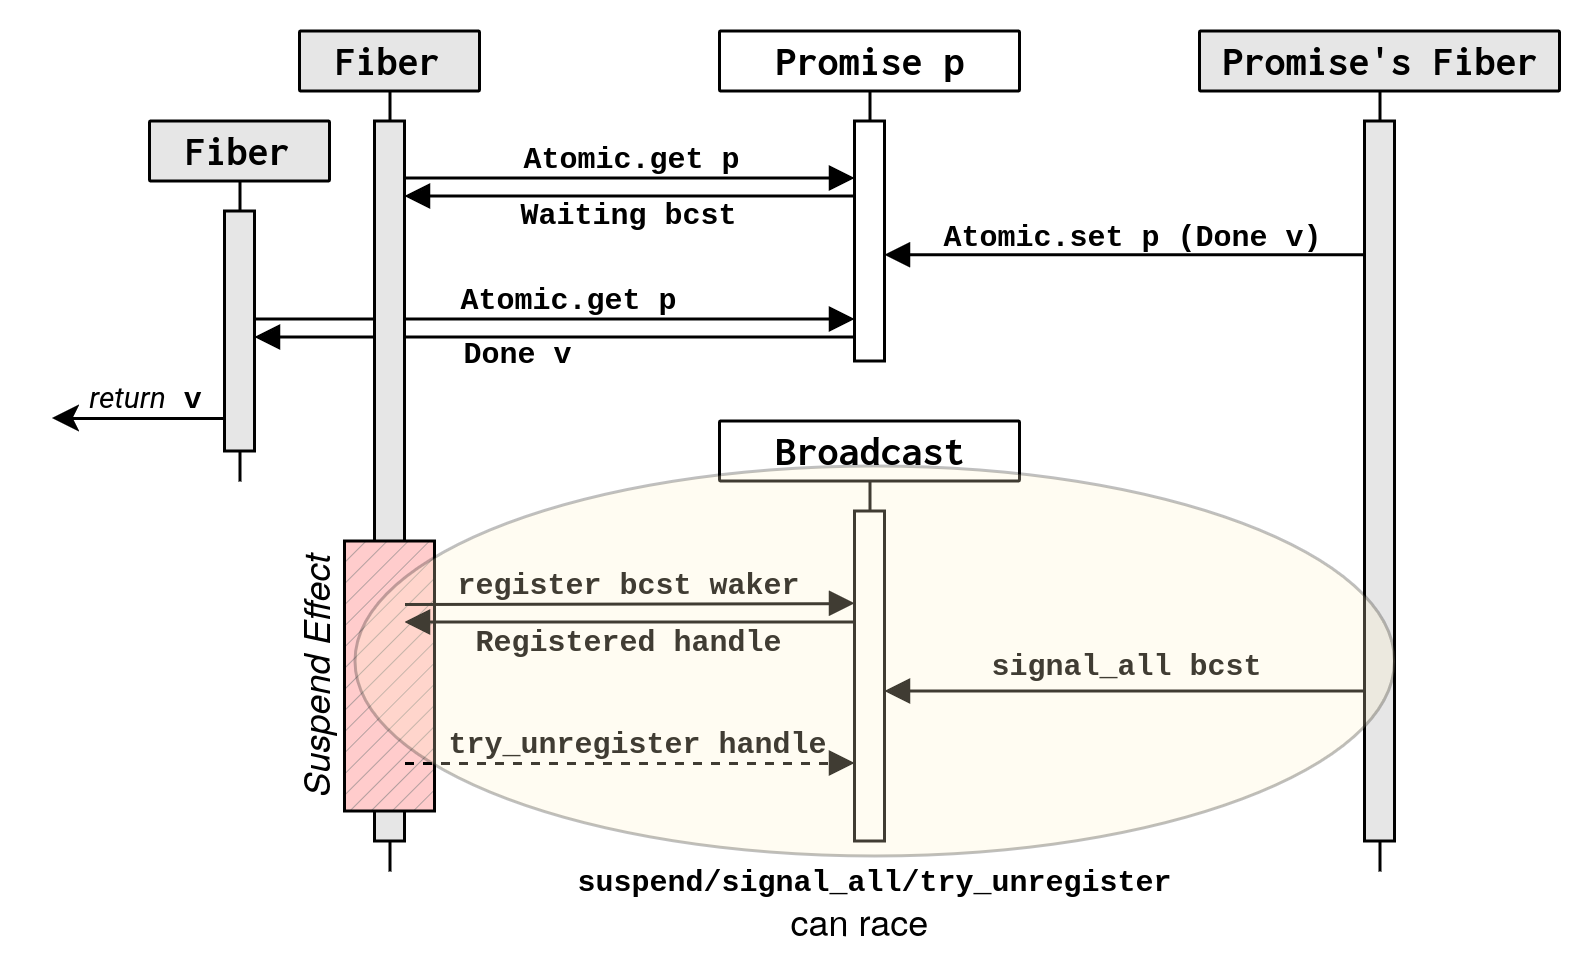
\includegraphics[width=\textwidth]{CQS_Outer_Atomic.png}
  \caption{Usage of broadcast in the context of a promise.}
  \label{fig:cqs-usage}
\end{figure}

Note that because all operations are lock-free and fibers can run in different threads, there can be a race between concurrent \ocamlin{register}, \ocamlin{try_unregister}, and \ocamlin{signal_all} operations.
Possible interleavings and the necessity of the \ocamlin{try_unregister} were explained in section~\ref{sec:sched-impl-await}.

\subsection{Implementation and Logical Interface of Broadcast}
\label{sec:broadcast-impl}

% <!-- Some general information how CQS is implemented and the logical state describing the entire queue. -->

Like the original CQS, broadcast is implemented as a linked list of arrays (called segments) that contain \emph{cells}\footnote{Using segments instead of single cells in the linked list is an optimization to amortize the linear runtime of linked list operations.}.
There are two pointers pointing to the beginning and end of the active cell range, the signal pointer and the register pointer, and cells not reachable from either pointer are garbage collected.
There is a set of operations for manipulating the linked list and pointers to implement the higher-level functionality, but they are not part of the public API, so we do not focus on them.
Each cell is a container for one callback and the logical state of the broadcast tracks the current state of all existing cells.
The possible states for a single cell are shown in figure~\ref{fig:cqs-cell-states}, where the arrows are annotated with the operation that causes a state transition.

The state of a cell is initialized to \textbf{EMPTY} when it is reached by the register pointer\footnote{In the original CQS, a cell can also be initialized when it is reached by the signal pointer, but in broadcast the signal pointer never overtakes the register pointer.}.
When a \ocamlin{register} and \ocamlin{signal_all} operation happen concurrently, they race to set the value of the empty cell.
If the \ocamlin{signal_all} operation wins, it writes a token value into the cell and the state becomes \textbf{SIGNALLED}.
The \ocamlin{register} operation can then read the token and invoke its callback directly.
The state is thus \textbf{INVOKED}.
If instead the \ocamlin{register} operation wins the race, it writes the callback into the cell, so the state takes the right path to \(\textbf{CALLBACK}_\textbf{waiting}\).
Then there can be another race between concurrent \ocamlin{try_unregister} and \ocamlin{signal_all} operations.
Both try to overwrite the callback with a token value, which changes the state to \(\textbf{CALLBACK}_\textbf{invoked}\) or \(\textbf{CALLBACK}_\textbf{unregistered}\), respectively, depending on the winner.
A \ocamlin{signal_all} ignores a lost race against \ocamlin{try_unregister} because it should disregard the callback in question, while \ocamlin{try_unregister} returns the outcome of the race as a boolean value.
If it won, then the caller knows that it is now responsible to invoke the callback itself.

\begin{figure}[ht]
  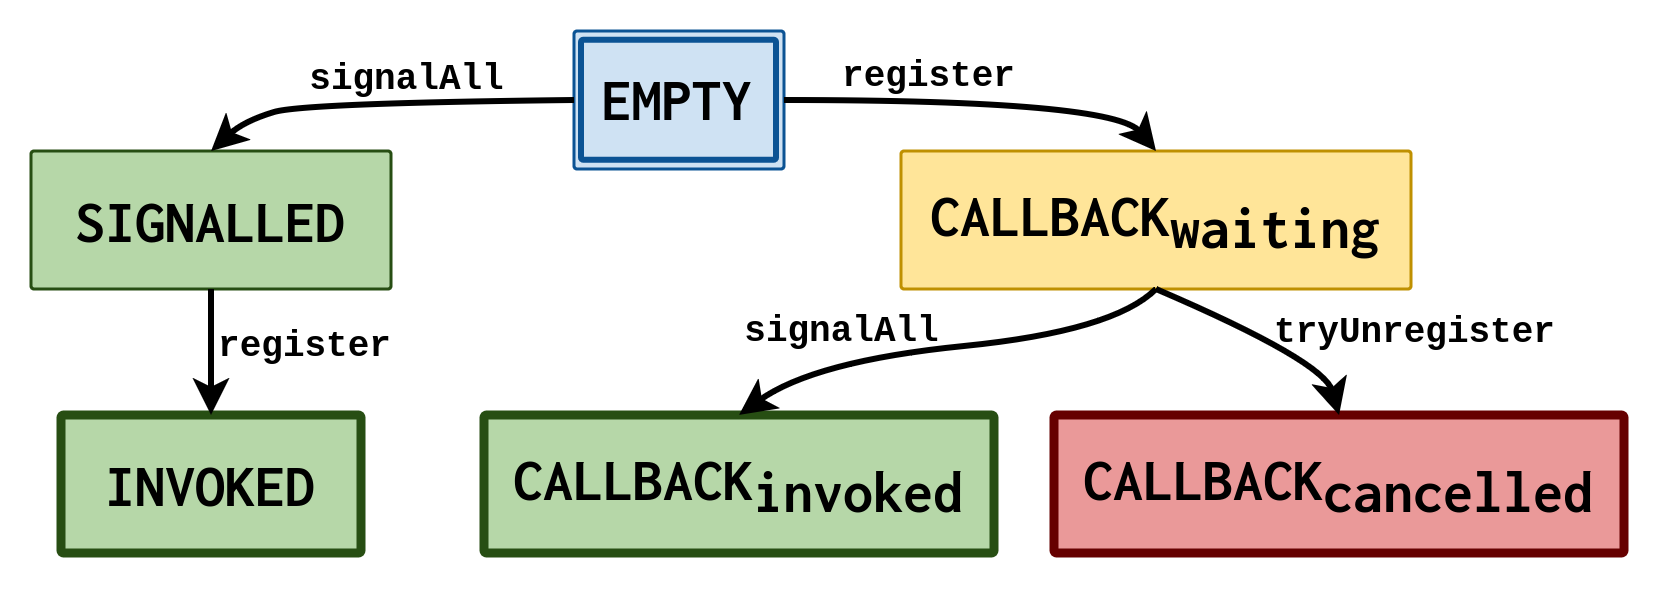
\includegraphics[width=\textwidth]{Cell_States.png}
  \caption{State transition diagram for a single cell.}
  \label{fig:cqs-cell-states}
\end{figure}

\subsection{Verification of Broadcast}
\label{sec:broadcast-spec}

Note that the specifications of all broadcast operations obey the empty protocol because the code does not perform any effects.
For all three operations, the Eio implementation and specification differs from what is already verified in the original CQS (e.g. due to some reordered instructions or a different control flow).
However, the specifications of the underlying operations for manipulating cell pointers are modular enough to allow us to prove the new specifications for \ocamlin{Broadcast.create}, \ocamlin{Broadcast.register}, and \ocamlin{Broadcast.try_unregister}.

As for \ocamlin{Broadcast.signal_all}, Eio implements this function by atomically increasing the signal pointer by the number \(n\) of registered callbacks and then processing all \(n\) cells between the old and new pointer position.
Because of technical differences in handling these pointers between the original CQS implementation of the paper~\cite{koval2023cqs} and the broadcast implementation of Eio we opted to verify a different implementation of \ocamlin{Broadcast.signal_all}, that increments the signal pointer \(n\) times in a loop and processes a single cell each time.
We argue this does not change the observable behaviors of the function since we ensure that it can only be called once.

\subsubsection{\ocamlin{Broadcast.create}}
\label{sec:broadcast-spec-create}

The only precondition to create a new broadcast is the proposition \(inv\_heap\_inv\).
This is a piece of ghost state defined by the Iris standard library that models invariant locations, which are locations that can always be read.
That means they cannot be explicitly deallocated and can only exist in a garbage-collected setting, like \ocf{}.
The implementation of the linked list uses this internally.

The function returns a broadcast instance \(bcst\), along with the persistent \(\gsIsBcst{}\; bcst\) proposition that shows the value actually is a broadcast.
We also obtain the unique resource \gssignal{}, which is held by the enclosing promise and allows calling the \ocamlin{Broadcast.signal_all} function once.

\[
  \inferrule[Spec-BroadcastCreate]
  {inv\_heap\_inv}
  {\ewp{create\; ()}{\bot}{bcst.\; \gsIsBcst{}\; bcst \ast \gssignal{}}}
\]

\subsubsection{\ocamlin{Broadcast.register}}
\label{sec:broadcast-spec-suspend}

% For a \emph{register} operation the \emph{suspend permit} from the original CQS is not needed anymore since we do the \emph{enqueue registration} internally.
A register operation takes a callback \(cb\) and the associated resource \(\gsIsCb{}\; cb\; R\) which represents the permission to invoke the callback when a precondition \(R\) is fulfilled.
\(\gsIsCb{}\) is not persistent because the callback must be invoked only once.

\begin{align*}
  \gsIsCb{}\; cb\; R                            & \triangleq R \wand \ewp{cb\; ()}{\bot}{\top}                                                                    \\
  \emph{isBroadcastRegisterResult}\; r\; cb\; R & \triangleq \begin{aligned}[t]
                                                                      & (\ulcorner r = Invoked \urcorner)                                                           \\
                                                               \vee\; & (\ulcorner r = Registered\; h \urcorner \ast \emph{isBroadcastRegisterHandle}\; h\; cb\; R)
                                                             \end{aligned} \\
  \emph{isBroadcastRegisterHandle}              & : Val \to Val \to iProp \to iProp
\end{align*}

The \ocamlin{Broadcast.register} function tries to insert a callback into the next cell designated by the register pointer.
If it succeeds the function returns a \ocamlin{Registered handle} value that can be used by \ocamlin{Broadcast.try_unregister}.
But if the cell is already in the \textbf{SIGNALLED} state, the function immediately invokes the callback and returns an \ocamlin{Invoked} value.

\[
  \inferrule[Spec-BroadcastRegister]
  { \gsIsBcst{}\; bcst \ast \gsIsCb{}\; callback\; R }
  { \ewp{register\; bcst\; callback}{\bot}{r.\; \emph{isBroadcastRegisterResult}\; r\; callback\; R}}
\]

\subsubsection{\ocamlin{Broadcast.try_unregister}}
\label{sec:broadcast-spec-cance}

Given a handle \(h\) and the associated \(\textit{isBroadcastRegisterHandle}\; h\; cb\; R\) resource, \ocamlin{Broadcast.try_unregister} tries to cancel the registration of the callback.

If the callback had already been invoked by \ocamlin{Broadcast.signal_all} (i.e. the state is \(\textbf{CALLBACK}_\textbf{invoked}\)) the function returns \ocamlin{false} and no resources are returned to the caller.
Otherwise, the permission to invoke the callback \(\gsIsCb{}\; cb\) is returned.

\[
  \inferrule[Spec-BroadcastTryCancel]
  { \emph{isBroadcastRegisterHandle}\; h\; cb\; R }
  { \ewp{try\_unregister\; h}{\bot}{b.\; if\; b\; then\; \gsIsCb{}\; cb\; R\; else\; \top}}
\]

\subsubsection{\ocamlin{Broadcast.signal_all}}
\label{sec:broadcast-spec-signal-all}

To call \ocamlin{Broadcast.signal_all} the unique \(\gssignal{}\) resource is needed along with a persistent \(R\), so that it can be used to invoke multiple callbacks.
The function does not return any resources because its only effect is invoking an unknown number of callbacks, none of which return any resources themselves.

\[
  \inferrule[Spec-BroadcastSignalAll]
  { \gsIsBcst{}\; bcst \ast \always R \ast \gssignal{}}
  { \ewp{signal\_all\; bcst}{\bot}{\top} }
\]

\subsection{Changes from the Original CQS}
\label{sec:broadcast-spec-removed-features}

The original CQS supports multiple additional features like a synchronous mode for suspend and resume, and also a smart cancellation mode.
These features enlarge the state space of CQS and complicate the verification but are not used in Eio so when we ported the verification of CQS to our Eio development we removed support for these features.
This reduced the state space of a cell shown in figure~\ref{fig:cqs-cell-states-original} to a more manageable size when adapting the proofs.

\begin{figure}[ht]
  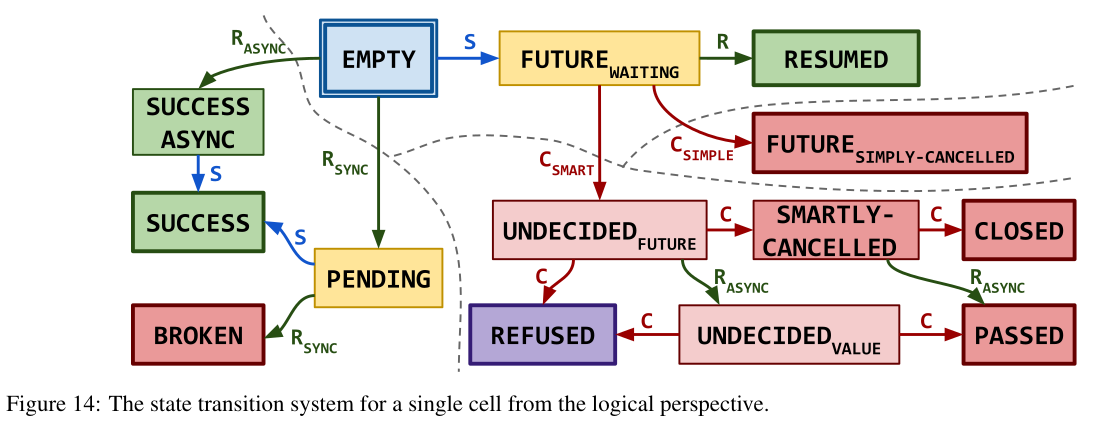
\includegraphics[width=\textwidth]{Cell_States_Original.png}
  \caption{Cell states in the original CQS from~\cite{koval2023cqs} (page 42).}
  \label{fig:cqs-cell-states-original}
\end{figure}

The part of the verification of the original CQS that we had to customize for Eio was originally 3600 lines of Coq code but -- due to these simplifications -- we could reduce it by approximately 1300 lines of Coq code.
Additionally, there are ~4000 lines of Coq code about lower-level functionality that we did not need to adapt when porting them to our development.

% The number of active cells \(n\) (i.e. the length of the queue) is tracked by the logical resource \(CQSState\; n\).
% In normal usage of CQS, the atomic variable of the outer synchronization construct would encode the length of the queue in its value and keep this resource in an associated invariant.
% Changing the length of the queue is done using \emph{enqueue} and \emph{dequeue registration} logical operations when opening this invariant.

% However, for promises the exact length of the queue is irrelevant because the \ocamlin{signal_all} operation will always set the length to 0.
% So in the adapted proof for Eio's broadcast we keep the \(CQSState\; n\) resource in the invariant of the broadcast itself.
% As a consequence we also move the \emph{enqueue} and \emph{dequeue registration} out of the public logical API because they are now done internally.

